\section{深入理解Ed25519}

\subsection{Ed25519概述}

Edwards-curve Digital Signature Algorithm (EdDSA)是定义在
(扭曲)爱德华曲线上Schnorr签名的变种签名机制.
Ed25519是Bernstein等人2011年在扭曲爱德华椭圆曲线Edwards25519 
(与蒙哥马利曲线Curve25519双向有理等价)上构建的签名机制\footnote{
Bernstein, Daniel J., Niels Duif, Tanja Lange, Peter Schwabe, and Bo-Yin Yang. 
"High-speed high-security signatures." 
In International Workshop on Cryptographic Hardware and Embedded Systems, 
pp. 124-142. Springer, Berlin, Heidelberg, 2011.
\url{https://link.springer.com/content/pdf/10.1007/978-3-642-23951-9_9.pdf}},
显著特点是高效安全,在保证128比特的安全强度的前提下
在2.4GHz的Intel Westmere (Xeon E5620) CPU上可以达到10万/秒的签名速度和7万/秒的验签速度.
RFC 8032\footnote{
RFC 8032. Edwards-Curve Digital Signature Algorithm (EdDSA).
\url{https://tools.ietf.org/html/rfc8032}}
中给出了EdDSA签名的具体规范,
并且给出了基于两条具体曲线Edwards25519和Edwards448的签名机制Ed25519和Ed448测试向量.
其中Edwards448是Mike Humberg构建的椭圆曲线,旨在提供224比特的安全强度.
值得注意的是, 2015年Bernstein对EdDSA签名机制进行了推广\footnote{
Bernstein, Daniel J., Simon Josefsson, Tanja Lange, Peter Schwabe, and Bo-Yin Yang. 
"EdDSA for more curves." Cryptology ePrint Archive 2015 (2015).
\url{https://eprint.iacr.org/2015/677.pdf}}
以使EdDSA签名机制可以适用于更多的椭圆曲线.
本文中,我们重点关注基于Edwards25519曲线的EdDSA的变种形式
\textsf{PureEdDSA}和\textsf{HashEdDSA}的签名机制:\textsf{Ed25519}和\textsf{Ed25519ph}.
RFC 8032中为了统一两个变种的定义,引入了预哈希函数(Prehash) \textsf{PH}的参数.
HashEdDSA是经典的先计算哈希值然后对哈希值计算签名的模式,也即对于任意长度的消息$m$,
\textsf{PH}都会输出固定长度的哈希值,例如\textsf{PH}可以定义为\textsf{SHA-512}: 
$\textsf{PH}(m) = \textsf{SHA-512}(m)$. PureEdDSA则直接对消息本身进行签名,
此时\textsf{PH}为恒等函数(Identity Function), 也即$\textsf{PH}(m) = m$.

EdDSA签名机制具有诸多良好的特性: 
1) 在各种平台上都可以高速实现; 2) 签名过程不需要外部随机数; 3) 能够有效抵抗侧信道攻击;
4) 公钥和签名值都较小,对于Ed25519而言公钥为32个字节签名值为64个字节;
5) 曲线上的点群运算是完备(Complete)的, 也即对于所有的点群中元素都成立, 计算时无需做额外的判断, 
意味着运算时不需要对不受信的外部值做昂贵的点的验证; 
6) EdDSA签名机制本身安全性不受哈希碰撞的影响,而ECDSA在出现哈希碰撞时会出现安全问题.

\subsection{EdDSA签名机制}

根据Bernstein等人在2015年对EdDSA签名机制的推广和RFC 8032中的规范, EdDSA签名机制有11个参数:
\begin{enumerate}
\item 
奇素数$p$: EdDSA所依赖的椭圆曲线构建在有限域$\F_p$上.
\item 
整数$b$满足$2^{b-1} > p$: EdDSA公钥为$b$比特,签名值为$2b$比特, $b$应为8的整数倍.
\item
有限域$\F_p$中元素的$b-1$比特的编码.
\item
可以产生$2b$比特输出的具有密码学安全强度的哈希函数\textsf{H}.
\item
$\F_p$中的二次非剩余$d$, $d$是椭圆曲线方程的参数,推荐选择尽可能接近零的值.
\item
$\F_p$中非零元素$a$, $a$是曲线方程参数, 推荐$p \mod 4=1$取$a=-1$, 否则取$a=1$.
\item 
基点$B \neq (0, 1)$并且$B \in E = \{(x,y) \in \F_p \times \F_p\ s.t.\ ax^2 + y^2 = 1 + dx^2y^2\}$.
\item
整数$c = 2$或$c = 3$, $2^c$是椭圆曲线的余因子(cofactor), EdDSA私钥为$2^c$的倍数.
\item
整数$n$满足$c \leq n < b$, 私钥为$n+1$比特,最高位为1 ($2^n$位),最低$c$位置零.
\item
奇素数$\ell$满足$\ell B = (0,1)$并且$2^c \times \ell = \# E$, 即$\ell$为椭圆曲线点群的阶(Order).
\item
预哈希函数\textsf{PH}, \textsf{PureEdDSA}和\textsf{HashEdDSA}对\textsf{PH}的定义不同.
\end{enumerate}
点群中的单位元为$(0,1)$,并且点群上的加法运算是完备的(Complete), 
也即对于任意的点$(x_1,y_1), (x_2, y_2)$都有
$$(x_1, y_1) + (x_2, y_2) = \left( \frac{x_1y_2 + x_2y_1}{1 + dx_1x_2y_1y_2}, 
\frac{y_1y_2 - ax_1x_2}{1-dx_1x_2y_1y_2}\right)$$

整数$s: 0 < s < \ell - 1$用小端法编码为$b$比特的字符串的过程记为$\textsf{Encode}(s)$.
而$(x,y)\in E$被编码为$b$比特的字符串,记为$\textsf{Encode}(x,y)$, $b$比特的编码
包含$y$的$(b-1)$比特的编码和1比特的符号位:如果$x$是负数, 则符号位为1, 否则为0.
根据这种编码方式可以立即确定$y$的值, $x$的值则需要通过方程
$x = \pm\sqrt{(y^2-1)/(dy^2-a)}$和符号位进行确定
(由于$d$是$\F_p$中的二次非剩余,所以分母$dy^2-a$不为零).
$x, y \in \F_p$, EdDSA签名体制中对有限域$\F_p$中的负数的定义为:
如果$x$的$(b-1)$比特的编码字符串比$-x$的$(b-1)$比特的编码字符串字典序更大
(Lexicographically Larger),则$x\in\F_p$是负数.
对于$p$是大的奇素数并且采用小端法编码的情形, $\F_p$中负数是所有的奇数$\{1, 3, 5, \ldots, q-2\}$.

EdDSA签名机制的私钥是$b$比特的值$k$, 记$\textsf{H}(k) = (h_0, h_1, \ldots, h_{2b-1})$.
$h_0, h_1, \ldots, h_{b-1}$确定了一个整数值$s$:
$$s =  2^n + \sum_{c \leq i < n}2^i h_i$$
整数值$s$决定公钥$\textsf{Encode}(A)$, 其中$A = sB$.
$h_b, h_{b+1}, \ldots, h_{2b-1}$用在签名值的计算过程中.
前面有提到, RFC 8032中根据预哈希函数\textsf{PH}的定义了给出了EdDSA的两个变种:
\textsf{PureEdDSA}和\textsf{HashEdDSA}, 由于两者的差异仅在于用\textsf{PH}处理
待签名消息$m$的结果不同,因此EdDSA可描述为:用\textsf{PureEdDSA}对$\textsf{PH}(m)$进行签名.

\textsf{PureEdDSA}对消息$m$计算签名值的结果$2b$比特的值
$\textsf{Encode}(R) || \textsf{Encode}(S)$: 
$$R = rB, S = \left(r + \textsf{H}\left(\textsf{Encode}(R) || 
\textsf{Encode}(A) || \textsf{PH}(m)\right)\cdot s \right) \mod \ell$$
其中$r = \textsf{H}(h_b || \ldots || h_{2b-1} || m)$并且被解释为小端法表示的$2b$比特的整数值.
用公钥值$\textsf{Encode}(A)$验证关于消息$m$的签名值$\textsf{Encode}(R) || \textsf{Encode}(S)$时,
首先需要从中解析出$A, R, S$的值,
并判定$A$和$R$是$E$中的元素并且$S$是集合$\{0, 1, \ldots, \ell-1\}$中的值,
然后判断如下等式是否成立
$$
(2^c \cdot S) B = 2^c  R + (2^c \cdot h) A,
\ \text{其中}\ h = \textsf{H}(\textsf{Encode}(R) || \textsf{Encode}(A) || \textsf{PH}(m))
$$
如果解析失败或者上述等式不成立,则判定为非法的签名值,否则判定为合法的签名值.
对消息$m$的EdDSA签名值的验证过程也即用\textsf{PureEdDSA}对$\textsf{PH}(m)$的签名值的验证过程.

\textsf{Ed25519}/\textsf{Ed25519ph}是基于扭曲爱德华曲线Edwards25519实例化的EdDSA签名机制, 
对应前述的EdDSA签名机制的11个参数分别为: 
\begin{enumerate}
\item 有限域$\F_p$的奇素数$p = 2^{255} - 19$.
\item 整数$b  = 256$, 也即\textsf{Ed25519}的公钥为256比特,签名值为512比特,注意到$2^{255} > p$.
\item $\F_p$中元素$\{0, 1, \ldots, p-1\}$的255比特编码是用小端法表示的整数值,最高位为零.
\item 
基于\textsf{SHA-512}\footnote{
RFC 6234: US Secure Hash Algorithms (SHA and SHA-based HMAC and HKDF).
\url{https://tools.ietf.org/pdf/rfc6234.pdf}}
的生成512比特输出的哈希函数$\textsf{SHA-512}(\textsf{dom2}(f, c) || x)$.
$f$是$flag$缩写,而$c$是$context$的缩写.
对于\textsf{Ed25519}, $\textsf{dom2}(f, c)$是空字符串, 也因此$f$和$c$的值无关紧要,
这样可以保证RFC 8032中定义的$\textsf{Ed25519}$与已有的$\textsf{Ed25519}$实现之间保持兼容. 
\textsf{Ed25519ctx}和\textsf{Ed25519ph}都可以带有额外的上下文参数$c$,至多为255个字节,
对于\textsf{Ed25519ctx}而言, $f = 0$, 对\textsf{Ed25519ph}而言, 则有$f = 1$. 
\item $\F_p$中的二次非剩余$d = -121665/121666$.
\item 由于$2^{255}-19 \mod 4 = 1$, 因此选取$\F_p$中的非零元素$a = -1$.
\item 基点$B$的横坐标\small{\textsf{0x216936d3cd6e53fec0a4e231fdd6dc5c692cc7609525a7b2c9562d608f25d51a}},
\normalsize
纵坐标为\small{\textsf{0x6666666666666666666666666666666666666666666666666666666666666658}}.
\normalsize
\item Edwards25519的余因子为8, 也因此整数参数$c = 3$.
\item $n = 254$.
\item Edwards25519的阶$\ell = 2^{252}+27742317777372353535851937790883648493$.
\item \textsf{Ed25519}的预哈希函数定义为\textsf{PH}为恒等函数, \textsf{Ed25519ph}的\textsf{PH}定义为\textsf{SHA-512}.
\end{enumerate}

由于Edwards25519的点坐标的值位于$\F_p$中, 根据$\F_p$中元素的255比特,可以用32字节的值
编码点$(x,y)$: 用255比特的值编码$y$的值,由于采用小端法编码,则32字节中的最后一个字节的最高位为零)
然后将$x$的最低比特赋值给最后一个字节的最高位即可. 这是因为最后一个字节的最高比特位是符号位,
符号位为1表示$x$为负值, 根据前述的关于$\F_p$中负数的定义可知, $\F_p$中的奇数均为负数, 
由于奇数的最低位为1, 所以将$x$的最低位赋值给符号位正好符合关于编码和负值的约定.

从32字节的编码中解码出点的值的步骤较编码复杂一些. 根据255比特的小端法编码可以直接得到$y$的值,
同时检查$y$的值在合理的范围之内并拒绝非法的值,而根据符号位可知$x$的最低位$x_0$.
根据$y$和曲线方程得到的$x^2 = (y^2-1) / (dy^2 + 1) (\mod p)$可以恢复$x$的值, 计算中会涉及到
域上的求逆运算和域上的开平方运算.求逆可以利用费马小定理$x^{-1} = x^{p-2} \mod p$
或者扩展的欧几里得算法完成.

记$u = y^2-1, v = dy^2 + 1$, 考虑根据$x^2 = u/v \mod p$计算$x$的值.
根据欧拉准则(Euler's Criterion),
如果$u/v$是$\F_p$中的二次剩余,则有$(u/v)^{(p-1)/2} \equiv 1 \mod p$;
如果$(u/v)^{(p-1)/2} \equiv -1 \mod p$, 则$x^2 = u/v \mod p$无解.
考虑$u/v$是$\F_p$中二次剩余的情况, 
注意到$2^{255}-19 \equiv 5 \mod 8$, 也即存在整数$k$使得$p = 8k + 5$.
由于$(u/v)^{(p-1)/2} \equiv 1 \mod p$, 则有$(u/v)^{(p-1)/4} \equiv \pm 1 \mod p$.
如果$(u/v)^{(p-1)/4} \equiv 1 \mod p$, 则$x = (u/v)^{k+1}\mod p$是一个解:
$$
x^2 \equiv (u/v)^{2(k+1)} \equiv (u/v)^{(p+3)/4} \equiv (u/v)^{(p-1)/4}\cdot (u/v) \equiv (u/v) \mod p 
$$
如果$(u/v)^{(p-1)/4} \equiv -1 \mod p$, 则$x = 2^{2k+1}(u/v)^{k+1}\mod p$是一个解:
$$
x^2 \equiv 2^{4k+2}(u/v)^{2k+2} \equiv 2^{\frac{p-1}{2}}(u/v)^{\frac{p+3}{4}} \equiv
 2^{\frac{p-1}{2}} (u/v)^{\frac{p-1}{4}}\cdot (u/v) \equiv -1 \cdot -1 \cdot (u/v) \mod p
$$
上式的推算过程中利用了2是$\F_p$中的二次非剩余这一事实以及欧拉准则.

根据上述过程,继续描述从32字节的编码中解码出点坐标值的过程,从$y$的值可以计算出$u, v$的值.
当$u/v$是$\F_p$中的二次剩余时,计算$x \equiv (u/v)^{(p+3)/8}\mod p$,
如果$x^2 \equiv (u/v) \mod p$, 则$x$是平方根,
如果$x^2 \equiv -(u/v)\mod p$, 则$2^{(p-1)/4} \cdot x$是平方根,
否则$u/v$不是$\F_p$中的二次剩余,意味着解码失败.
下一步则根据$x_0$的值选取正确的平方根,如果$x = 0$而$x_0 = 1$, 则解码失败.
如果$x_0 \neq x \mod 2$, 则$x = p-x$, 解码得到的点即为$(x,y)$.
注意在具体实现解码操作时,可以将求逆和求平方根的操作进行融合以简化运算,
$(u/v)^{(p+3)/8}\mod p$可以等价变换为:
$$
(u/v)^{(p+3)/8} = u^{\frac{p+3}{8}} v^{-\frac{p+3}{8}}
= u^{\frac{p+3}{8}} v^{(p-1)-\frac{p+3}{8}}
= u^{\frac{p+3}{8}} v^{\frac{7p-11}{8}}
= uv^3(uv^7)^{(q-5)/8} 
$$
而判断$x^2\equiv (u/v) \mod p$和$x^2 \equiv -(u/v) \mod p$可以等价变换为
$v \cdot x^2 \equiv u \mod p$和$v \cdot x^2 \equiv -u \mod p$.

\begin{figure}[h]
\centering
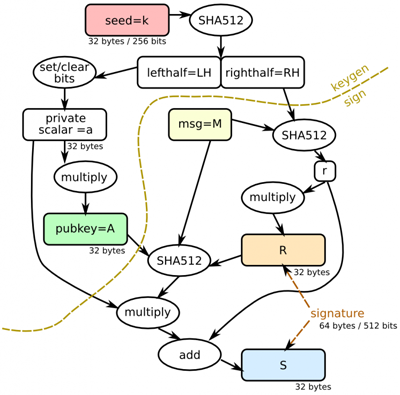
\includegraphics[width=.7\textwidth]{ed25519.png}
\caption{Ed25519签名过程}\label{fig-ed25519}
\end{figure}

与ECDSA签名机制中直接用私钥和基点进行点倍乘运算得到公钥值不同,
EdDSA签名机制中私钥和公钥之间的关系更为复杂,按照以下步骤进行,参见Figure~\ref{fig-ed25519}.
1) 用\textsf{SHA-512}计算32字节的私钥的512比特(64个字节)的哈希值,低32字节用于生成公钥;
2) 将32字节中第一个字节的最低3比特清零,最后一个字节的最高位清零,将最后一个字节的第二最高位置1;
3) 将设置之后的32字节的看做是小端法表示的整数,记为$s$, 计算$A = sB$;
4) $A$的编码$\textsf{Encode}(A)$是最终的公钥.


